\documentclass{article}
\usepackage[utf8]{inputenc}
\usepackage{amsmath,amssymb}
\usepackage{graphicx}
\usepackage{float}
\usepackage{subcaption}
\usepackage{geometry}
\geometry{
    a4paper,
    total={170mm,257mm},
    left=20mm,
    right=20mm,
    top=20mm,
}
\usepackage{listings} % code listings
\lstset{framextopmargin=0pt,frame=lines}
\lstset{
    language=Matlab,
    basicstyle=\footnotesize\ttfamily,
    breaklines=true,
    tabsize=4,
    keepspaces=true,
    columns=flexible,
    % backgroundcolor=\color[gray]{0.9},
    frame=single,
    breaklines=true,%
    morekeywords={matlab2tikz},
    keywordstyle=\color{blue},%
    morekeywords=[2]{1}, keywordstyle=[2]{\color{black}},
    identifierstyle=\color{black},%
    stringstyle=\color{mylilas},
    commentstyle=\color{mygreen},%
    showstringspaces=false,%without this there will be a symbol in the places where there is a space
    numbers=left,
    numberstyle={\tiny \color{black}},% size of the numbers
    numbersep=9pt, % this defines how far the numbers are from the text
    emph=[1]{for,end,break},emphstyle=[1]\color{red}, %some words to emphasise
    %emph=[2]{word1,word2}, emphstyle=[2]{style},
}
\usepackage{color} %red, green, blue, yellow, cyan, magenta, black, white
\definecolor{mygreen}{RGB}{28,172,0} % color values Red, Green, Blue
\definecolor{mylilas}{RGB}{170,55,241}

\usepackage{siunitx}
\newcommand{\e}[1]{\times 10^{#1}} % nicer scientific notation

\title{ENV-541 Sensor Orientation\\Lab 7 - Kalman Filtering with simulated GPS data: simple (a=0) model}
\author{Michael Spieler}
\date{November 9, 2018}

\begin{document}

\maketitle

% >> lab7
% Empirical std dev GPS:0.6666
% Empirical std dev KF filter:0.5125
% Final std dev KF predicted:0.5141
% >> lab7
% Empirical std dev GPS:0.6536
% Empirical std dev KF filter:0.5236
% Final std dev KF predicted:0.5141
% >> lab7
% Empirical std dev GPS:0.7538
% Empirical std dev KF filter:0.5982
% Final std dev KF predicted:0.5141
% >> lab7
% Empirical std dev GPS:0.6751
% Empirical std dev KF filter:0.4891
% Final std dev KF predicted:0.5141
% >> lab7
% Empirical std dev GPS:0.6550
% Empirical std dev KF filter:0.4877
% Final std dev KF predicted:0.5141

\section*{Plots}

Figure \ref{fig:traj} compares the true trajectory with the noisy GPS measurments and the estimated position for one realizations.

\begin{figure}[H]
    \centering
    \begin{subfigure}[t]{0.8\textwidth}
        \centering
        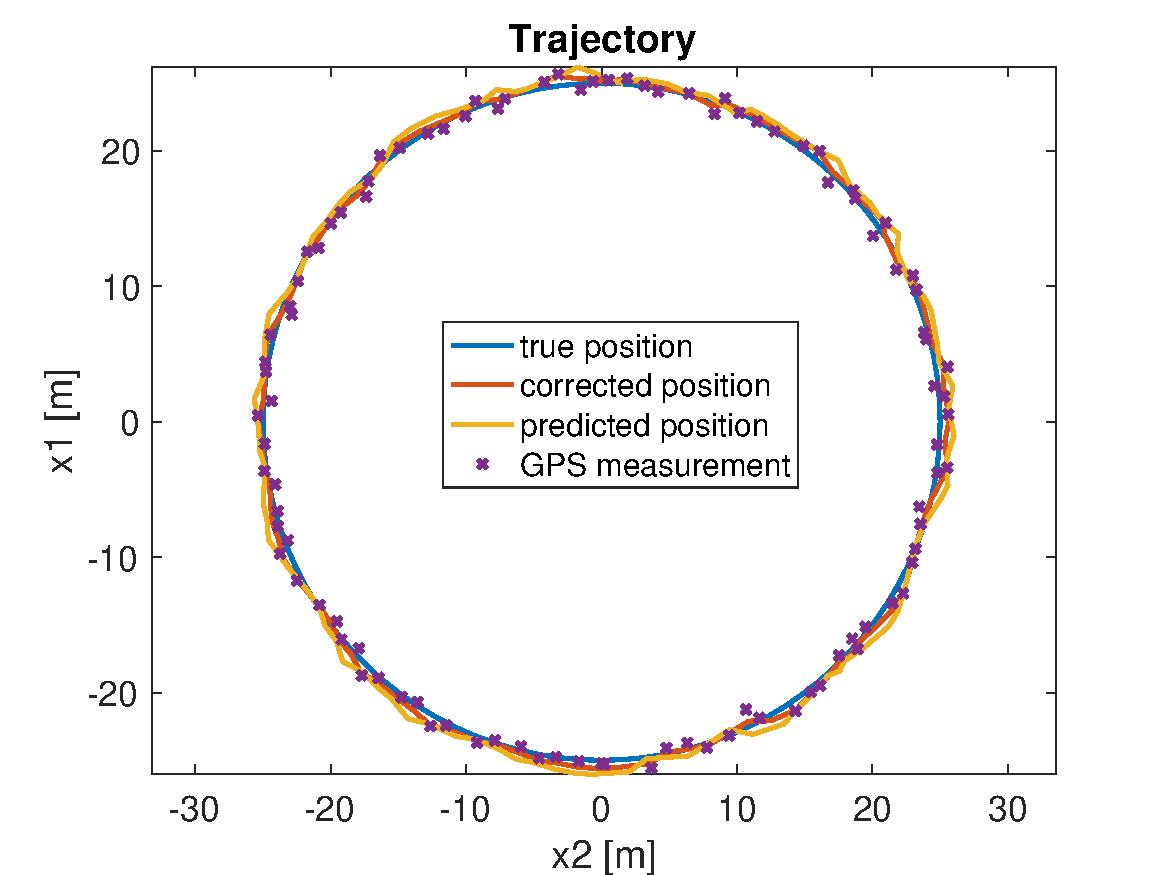
\includegraphics[width=\textwidth]{traj}
    \end{subfigure}
    \caption{Trajectory compared with measurements and KF estimate.}
    \label{fig:traj}
\end{figure}


\begin{figure}[H]
    \centering
    \begin{subfigure}[t]{0.49\textwidth}
        \centering
        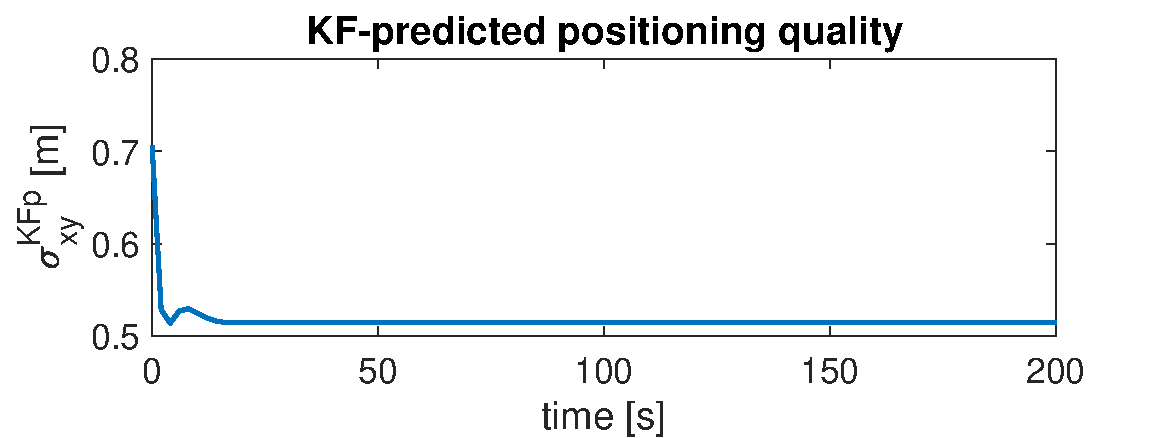
\includegraphics[width=\textwidth]{1_sigma_KF}
        \caption{Realization 1}
    \end{subfigure}
    ~
    \begin{subfigure}[t]{0.49\textwidth}
        \centering
        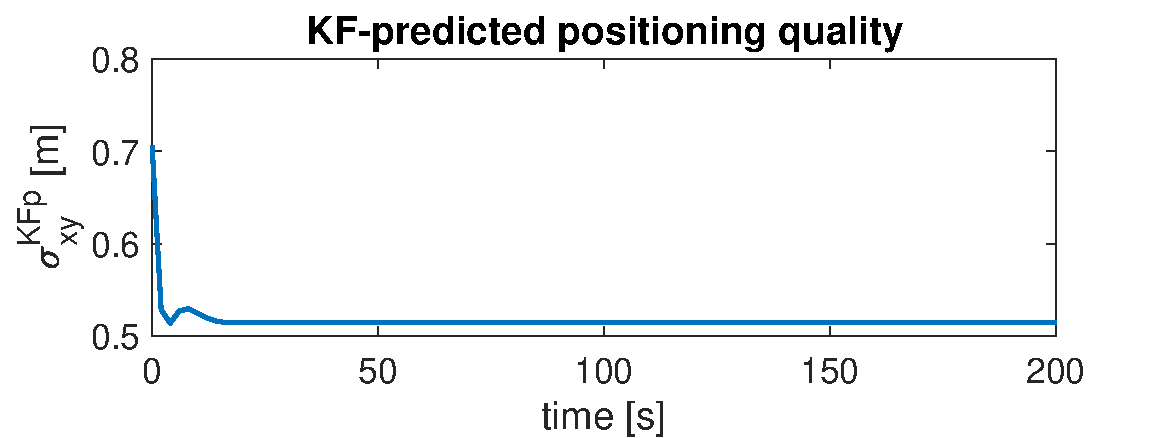
\includegraphics[width=\textwidth]{2_sigma_KF}
        \caption{Realization 2}
    \end{subfigure}
    ~
    \begin{subfigure}[t]{0.49\textwidth}
        \centering
        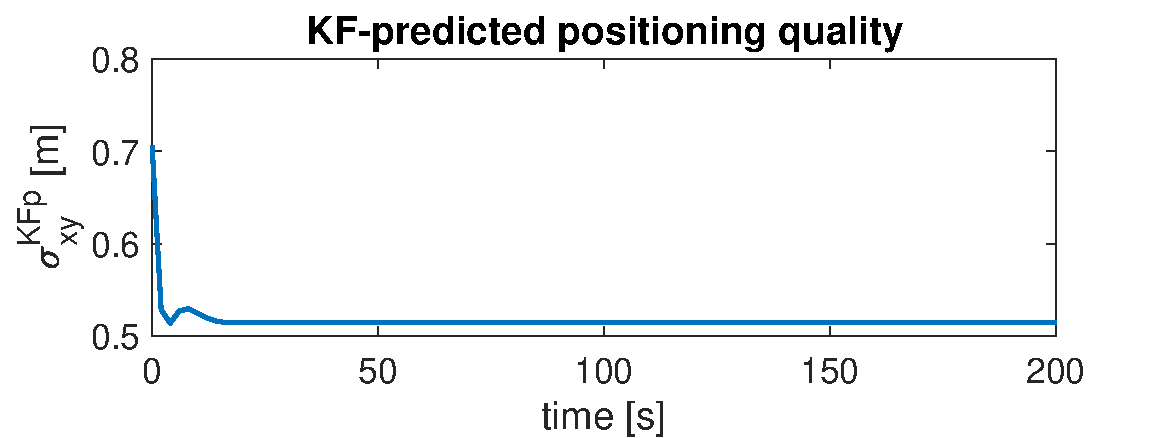
\includegraphics[width=\textwidth]{3_sigma_KF}
        \caption{Realization 3}
    \end{subfigure}
    ~
    \begin{subfigure}[t]{0.49\textwidth}
        \centering
        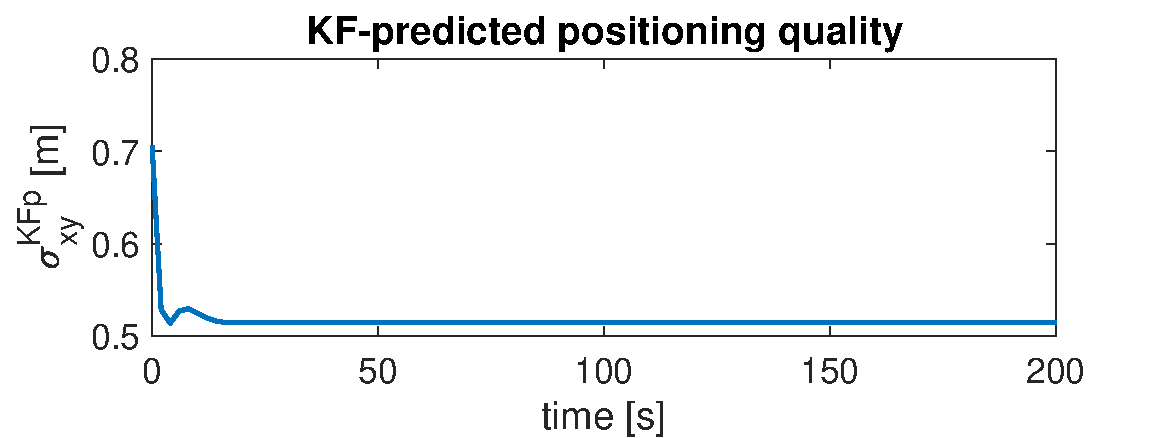
\includegraphics[width=\textwidth]{4_sigma_KF}
        \caption{Realization 4}
    \end{subfigure}
    ~
    \begin{subfigure}[t]{0.49\textwidth}
        \centering
        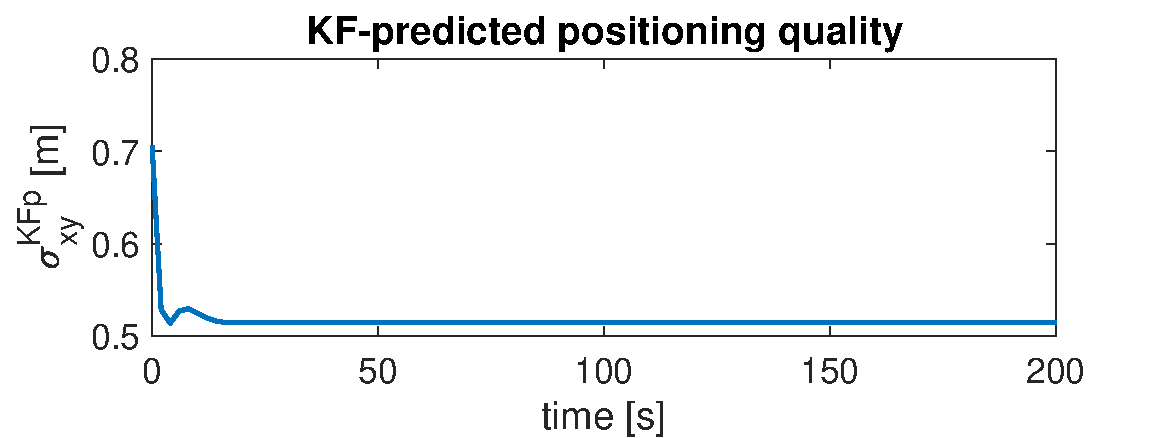
\includegraphics[width=\textwidth]{5_sigma_KF}
        \caption{Realization 5}
    \end{subfigure}
    \caption{evolution of the KF-predicted position quality.
            It is stable after 20s (10 updates).
            Note that all realizeaitons are identical.}
    \label{fig:error_gyro}
\end{figure}


\begin{figure}[H]
    \centering
    \begin{subfigure}[t]{0.49\textwidth}
        \centering
        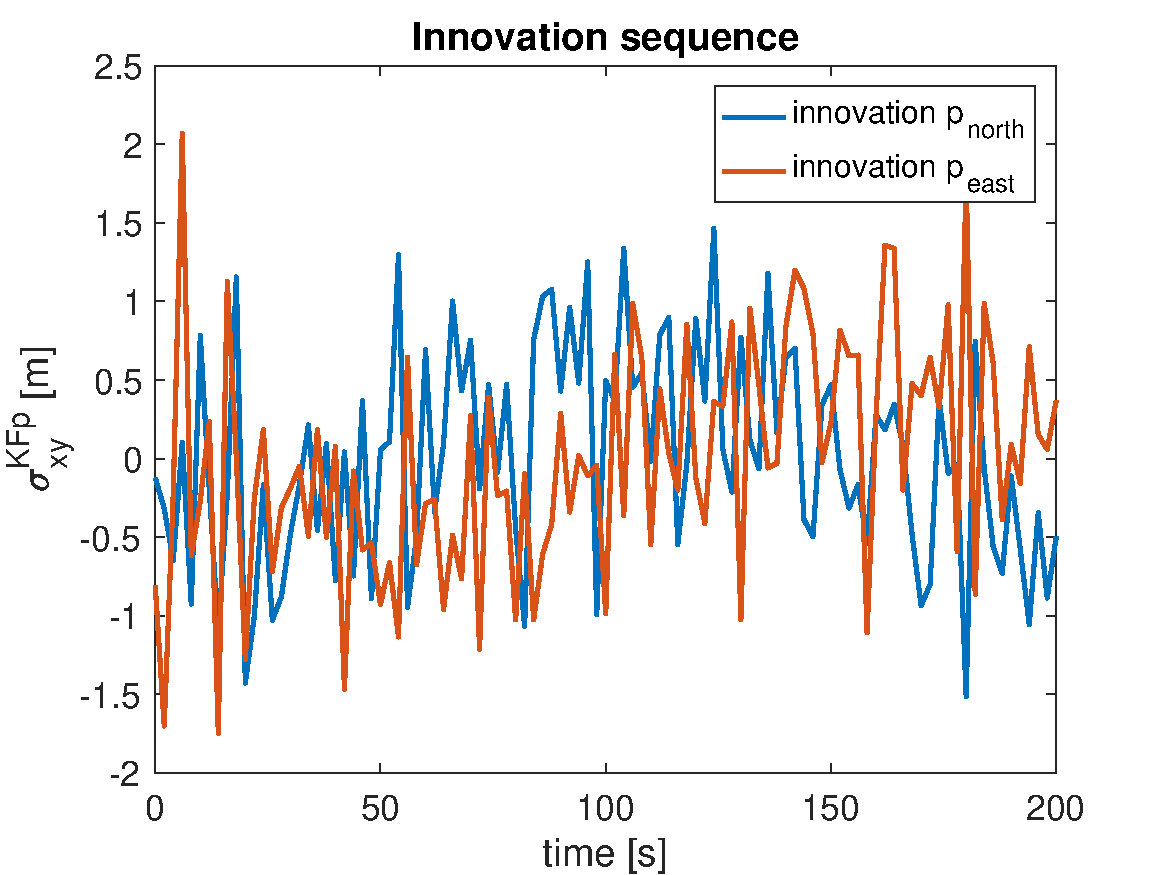
\includegraphics[width=\textwidth]{1_innovation}
        \caption{Realization 1}
    \end{subfigure}
    ~
    \begin{subfigure}[t]{0.49\textwidth}
        \centering
        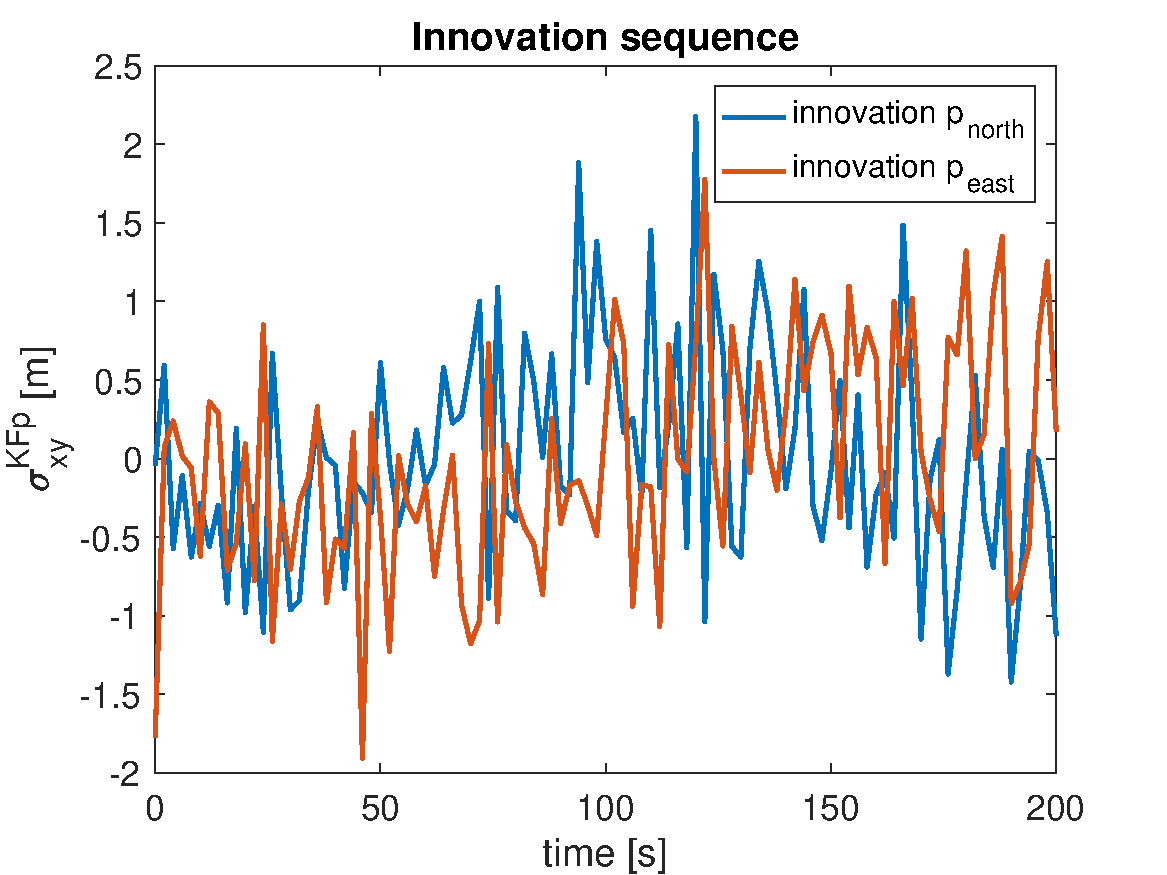
\includegraphics[width=\textwidth]{2_innovation}
        \caption{Realization 2}
    \end{subfigure}
    ~
    \begin{subfigure}[t]{0.49\textwidth}
        \centering
        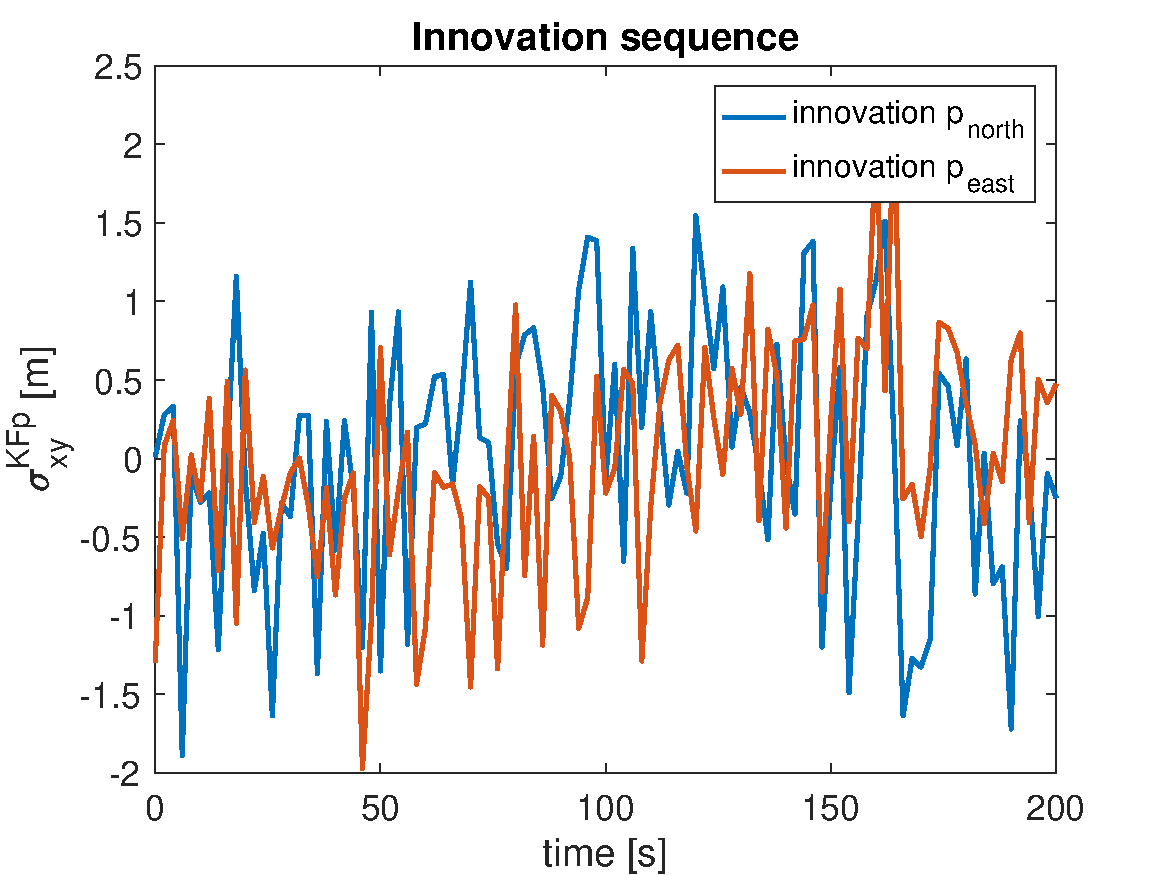
\includegraphics[width=\textwidth]{3_innovation}
        \caption{Realization 3}
    \end{subfigure}
    ~
    \begin{subfigure}[t]{0.49\textwidth}
        \centering
        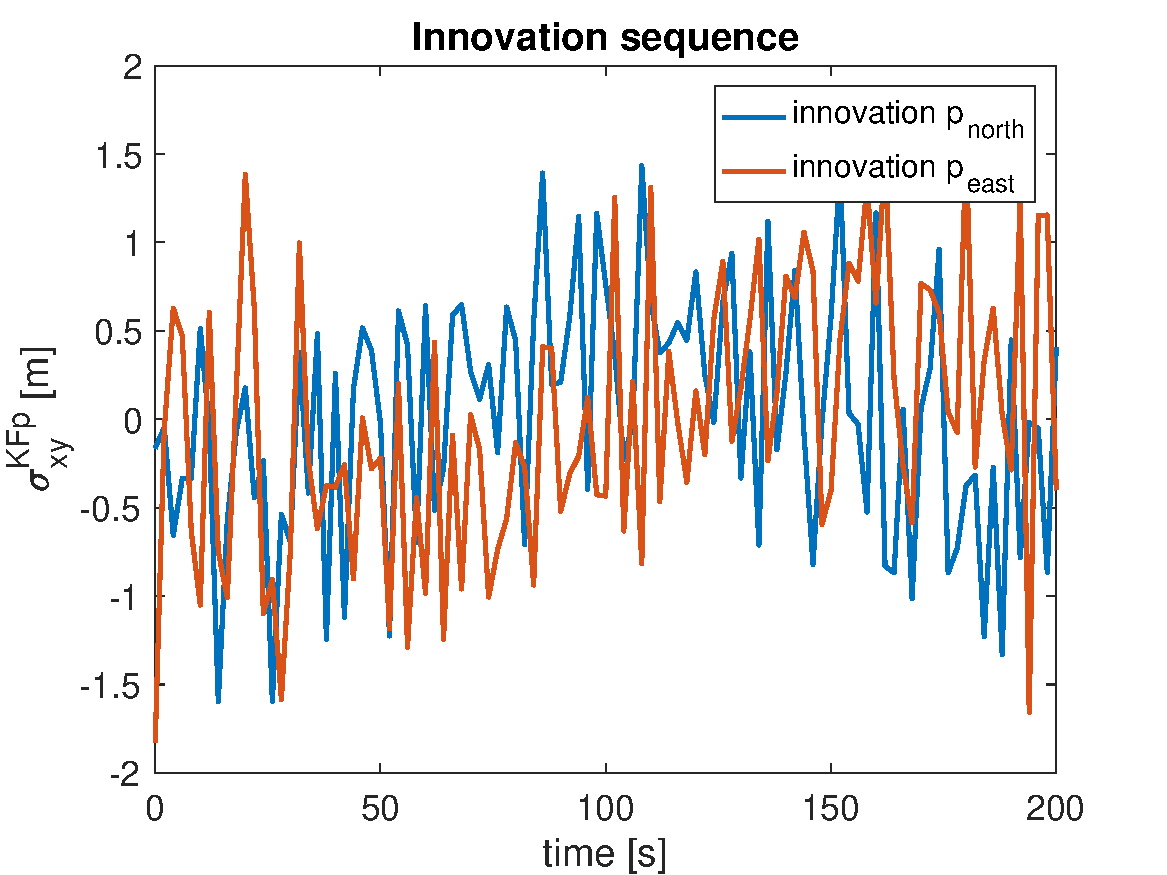
\includegraphics[width=\textwidth]{4_innovation}
        \caption{Realization 4}
    \end{subfigure}
    ~
    \begin{subfigure}[t]{0.49\textwidth}
        \centering
        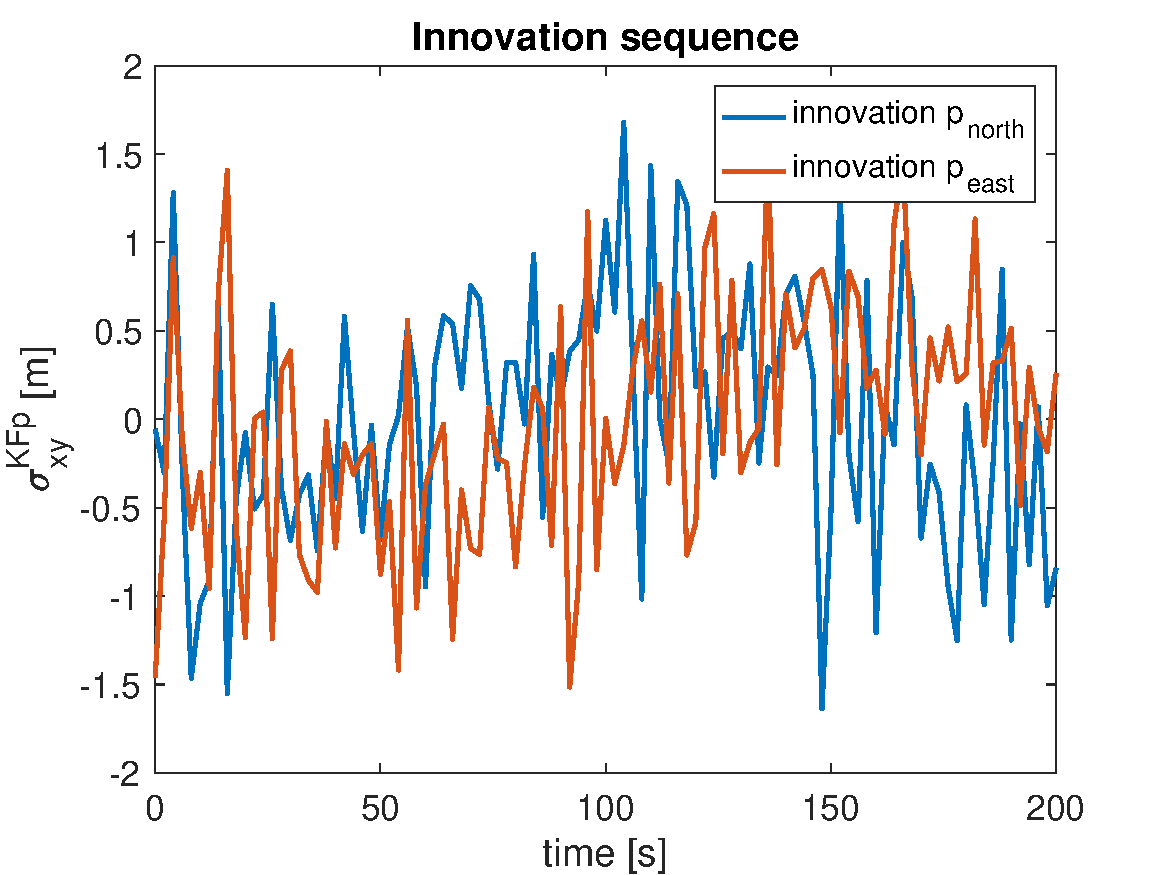
\includegraphics[width=\textwidth]{5_innovation}
        \caption{Realization 5}
    \end{subfigure}
    \caption{Evolution of the innovations}
    \label{fig:error_gyro}
\end{figure}

\newpage

Table \ref{tab:std_dev} summarizes the different accuracy estimates from the 5 realizations.

\begin{table}[h]
\centering
\begin{tabular}{lllllll}
Realizations  & 1 & 2 & 3 & 4 & 5 & mean\\
\hline
$\sigma_{xy}^{GPS_{emp.}}$ & $0.6666 \si{m}$ & $0.6536 \si{m}$ & $0.7538 \si{m}$ & $0.6751 \si{m}$ & $0.6550 \si{m}$ & $\mathbf{0.6808 \si{m}}$\\
$\sigma_{xy}^{KF_{emp.}}$  & $0.5125 \si{m}$ & $0.5236 \si{m}$ & $0.5982 \si{m}$ & $0.4891 \si{m}$ & $0.4877 \si{m}$ & $\mathbf{0.5222 \si{m}}$\\
$\sigma_{xy}^{KF_{p}}$(final) & $0.5141 \si{m}$ & $0.5141 \si{m}$ & $0.5141 \si{m}$ & $0.5141 \si{m}$ & $0.5141 \si{m}$ & $\mathbf{0.5141 \si{m}}$
\end{tabular}
\caption{Accuracy estimates from different realizations.}
\label{tab:std_dev}
\end{table}

\section*{Questions}

\subsubsection*{I. What is the true overall improvement of the positioning accuracy by the filtering
(i.e. through comparing $\sigma_{xy}^{KF_{emp.}}$ versus $\sigma_{xy}^{GPS_{emp.}}$).}

We gain in 0.15m of accuracy, which is more than $20\%$ improvement.
Also, we have an estimate of the accuracy.

\subsubsection*{II. How many measurements does it take to stabilize the predicted accuracy in position?}

Reading form the plotted KF-predicted positioning quality $\sigma_{xy}^{KF_{p}}$ it takes about 10 measurements (20 seconds) to stabilize (within $0.1\%$).

\subsubsection*{III. Does the evolution of the predicted positioning accuracy depend on the actual measurements?
If yes, why is that? If no, why is that?}

No, it does not depend on the actual measurements.
The stable (final) $\sigma_{xy}^{KF_{p}}$ is the same for all realizations.
This is easily explained when looking at the Kalman filter algorithm.
The covariance matrix P does not depend on the measurement z.

\subsubsection*{IV. How well does the empirically estimated position accuracy ( $\sigma_{xy}^{KF_{emp.}}$)
correspond to the anticipated/predicted accuracy ( $\sigma_{xy}^{KF_p}$ ) and which parameters
of the filter would you suggest modifying to improve the agreement?}

The empirically estimated position accuracy ($\sigma_{xy}^{KF_{emp.}}$)
is similar but slightliy bigger than the anticipated/predicted accuracy
$\sigma_{xy}^{KF_p}$.
Changing the motion model might improve the estimation.
Increasing the motion model uncertainty $\sigma_{\dot{v}}$ will make the predicted uncertainty bigger.

\newpage
\section*{Code}
\lstinputlisting{../lab7.m}

\end{document}
